\chapter{Conclusioni}
Al termine dello sviluppo si è riusciti ad ottenere un classificatore di ADLs in grado di interagire con una applicazione Android.

\vspace{5mm} %5mm vertical space

Prendendo in considerazione le sole 3 attività scelte per la classificazione (camminata, corsa e salti) su cui abbiamo testato il riconoscimento 
e la partizione di cui abbiamo mostrato i risultati grafici durante la trattazione, siamo riusciti ad ottenere un buon riconoscimento 
delle attività con \textit{solamente} poco più di 250 mila record di dati.

\vspace{5mm} %5mm vertical space

L'aggiunta di ulteriori attività comporterebbe logicamente l'esigenza di incrementare le informazioni di apprendimento per mantenere 
invariata l'accuratezza del riconoscimento. Reputo entrambi questi passaggi fondamentali per l'utilizzo del 
classificatore nel mondo reale, oltre che per il riconoscimento di una quantità maggiore di ADLs.

\subsection*{Ottimizzazioni future}
L'intero sistema può essere ulteriormente migliorato. 
Sono stati ipotizzati dei possibili scenari per una futura ottimizzazione del sistema.

\subsubsection{Disponibilità offline}
Così come è stato presentato e realizzato il sistema dipende completamente dalla connessione di rete, nonché dalla comunicazione costante con il server 
durante una qualsiasi attività che preveda la raccolta dei dati.
Un'opportuna ottimizzazione sarebbe quella di rendere il tutto funzionante anche in assenza di connessione.

\vspace{5mm} %5mm vertical space
L'applicazione potrebbe raccogliere i dati inerziali di apprendimento all'interno di un database locale e procedere all'invio al server 
anche in un secondo momento. La fase di riconoscimento invece potrebbe avvenire all'interno del dispositivo con 
l'utilizzo di Tensorflow Lite \cite{tensorflow_lite} e dei modelli pre-allenati scaricati dal server in precedenza.

\vspace{5mm} %5mm vertical space
Con questa ottimizzazione il server continuerà ad avere una funzione chiave nell'intero sistema (l'aggregazione dei dati, la 
generazione dei modelli e la conversione degli stessi nel formato adatto), ma si perde la necessità di avere un collegamento costante.

\begin{figure}[H]
    \centering
    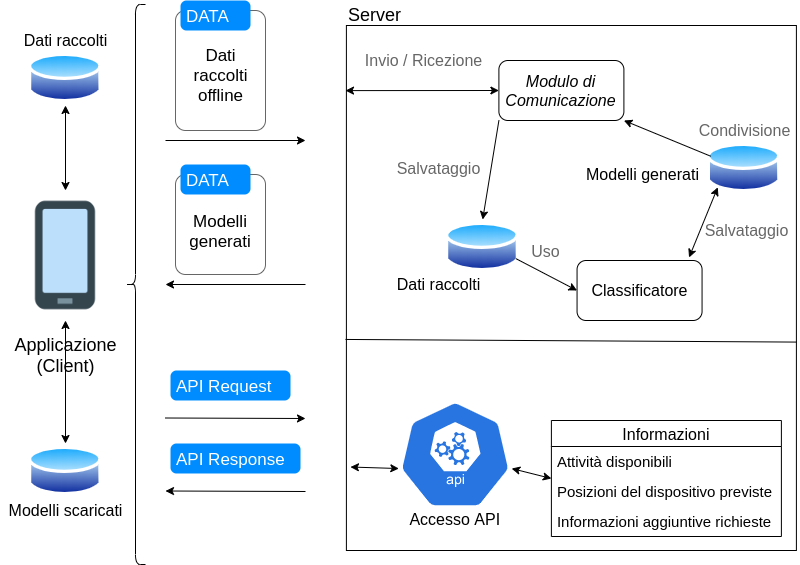
\includegraphics[scale = 0.56]{assets/images/future/offline.png}
    \caption{Ottimizzazione del progetto per l'utilizzo offline}
    \label{fig:future_overview}
\end{figure}

\subsubsection{Aggregazione dei sensori}
Al momento il riconoscimento delle attività si basa sull'utilizzo separato delle informazioni raccolte dai diversi sensori inerziali.
Uno dei partizionamenti visti sul set di dati completo è appunto quello riguardante il sensore utilizzato.

\vspace{5mm} %5mm vertical space

Una seconda ottimizzazione fattibile sarebbe quella di generare un modello che utilizzi contemporaneamente le caratteristiche di uno e dell'altro sensore.
Questo modello sarà in aggiunta ai precedenti. I modelli al momento presenti non saranno completamente rimpiazzati poiché potrebbero 
tornare utili nell'eventualità che un singolo sensore sia disabilitato o non presente sul dispositivo di acquisizione.

\subsubsection{Dati fisici}
Il classificatore sviluppato si basa principalmente sui dati inerziali senza tener conto in alcun modo dell'utente 
che sta eseguendo l'attività.

\vspace{5mm} %5mm vertical space

Una terza ottimizzazione possibile sarebbe quella di richiedere all'utente, tramite il modulo già sviluppato, maggiori 
informazioni riguardo la sua fisicità ed assegnare a queste un peso nella classificazione.
Dato che in alcune attività le caratteristiche fisiche potrebbero avere un rilievo, un miglioramento del genere porterebbe ad 
ottenere una maggior accuratezza dei risultati.